P kontrolör
\begin{equation}
    F(s)=k
\end{equation}
olmak üzere kapalı çevrim transfer fonksiyonu 
\begin{equation}
\begin{split}
    T(s)&=\frac{F(s)G(s)}{1+F(s)G(s)}\\
    &=\frac{k\frac{1}{s^2+s+1}}{1+k\frac{1}{s^2+s+1}}\\
    &=\frac{k}{s^2+s+1+k}
\end{split}
\end{equation}
olarak elde edilmektedir. Tasarım için 
\begin{equation}
\begin{split}
    1&=8\\
    1+k&=45.7844
\end{split}
\end{equation}
eşitliği çözülmelidir. Görüldüğü üzere çözüm mevcut değildir. Sadece aşım için çözülmek istenirse, \begin{equation}
\begin{split}
    p(s)&=s^2+2\zeta \omega_n s+\omega_n^2\\
    &=s^2+1.1824\omega_n s+\omega_n^2
\end{split}
\end{equation}
kullanılarak 
\begin{equation}
\begin{split}
    1.1824\omega_n&=8\\
    1+k&=\omega_n^2
\end{split}
\end{equation}
probleminin çözümü $\omega_n=0.8458$ ve $k=-0.2846$ elde edilmektedir. Kapalı çevrim transfer fonksiyonu
\begin{equation}
    T(s)=\frac{-0.2846}{s^2 + s + 0.7154}
\end{equation}
olarak hesaplanmaktadır. Basamak yanıtı Şekil~\ref{fig:p_kontrol} ile gösterilmektedir.
\begin{figure}[!htb]
    \centering
    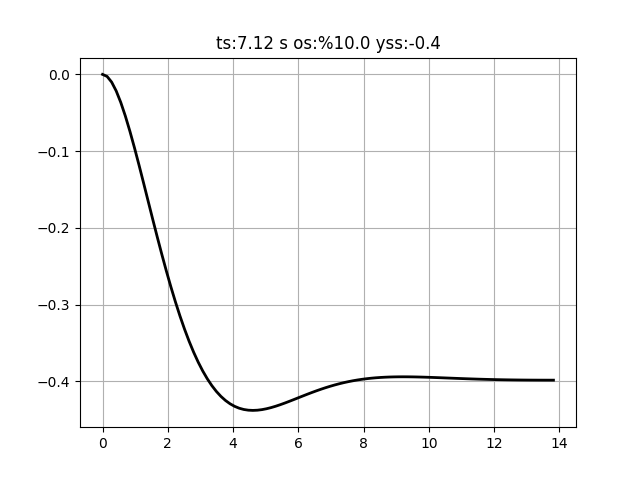
\includegraphics[width=0.75\textwidth]{p_kontrol}
    \caption{P kontrolör}
    \label{fig:p_kontrol}
\end{figure}